\documentclass[10pt,twocolumn,letterpaper]{article}

\usepackage{cvpr}
\usepackage{times}
\usepackage{epsfig}
\usepackage{graphicx}
\usepackage{amsmath}
\usepackage{amssymb}

% Include other packages here, before hyperref.

% If you comment hyperref and then uncomment it, you should delete
% egpaper.aux before re-running latex.  (Or just hit 'q' on the first latex
% run, let it finish, and you should be clear).
\usepackage[pagebackref=true,breaklinks=true,letterpaper=true,colorlinks,bookmarks=false]{hyperref}

\cvprfinalcopy % *** Uncomment this line for the final submission

\def\cvprPaperID{****} % *** Enter the CVPR Paper ID here
\def\httilde{\mbox{\tt\raisebox{-.5ex}{\symbol{126}}}}

% Pages are numbered in submission mode, and unnumbered in camera-ready
\ifcvprfinal\pagestyle{empty}\fi
\begin{document}

%%%%%%%%% TITLE
\title{Characterizing Redundancy in Natural Images}

\author{Niru Maheswaranathan\\
Stanford University\\
\textit{nirum@stanford.edu}
% For a paper whose authors are all at the same institution,
% omit the following lines up until the closing ``}''.
% Additional authors and addresses can be added with ``\and'',
% just like the second author.
% To save space, use either the email address or home page, not both
%Second Author\\
%Institution2\\
%First line of institution2 address\\
%{\tt\small secondauthor@i2.org}
}

\maketitle
\thispagestyle{empty}

%%%%%%%%% ABSTRACT
\begin{abstract}
The space of natural images is both high-dimensional and has striking non-Gaussian, higher-order statistical structure. It has been argued on information theoretic grounds that much of early visual processing consists of removing statistical regularities in visual input, in what is known as the redundancy reduction hypothesis. A key part of understanding the redundancy of natural scenes is understanding the entropy of image patches. Entropy allows us to quantify the information content of image patches, and bounds optimal compression schemes. This project aims to characterize the redundancy of natural images by quantifying the entropy of both the raw ensemble of images as well as other generative models of natural images.
\end{abstract}

%%%%%%%%% BODY TEXT
%\noindent\large\textbf{Future Distribution Permission}\\
%\indent The author(s) of this report give permission for this doc- ument to be distributed to Stanford-affiliated students taking future courses.

%\section{Problem statement}

\section{Motivation}
It has long been argued \cite{barlow} that the human visual system has evolved to efficiently process the statistical structure of natural images. This suggests that computer vision systems can also be tuned to the structure of natural images. A useful metric for quantifying the redundancy in the distribution of image patches is the entropy of the distribution. Entropy can be thought of as a measure of the information content of a distribution, therefore, the entropy of the distribution of natural scenes bounds the amount of information available to vision systems (either man-made or in nature). Entropy also provides a lower bound on the number of bits needed for compression, thus knowledge of the entropy of natural images gives us an absolute threshold with which to compare compression schemes.

%designed given this statistical structure. One example of where knowledge of the statistical structure of natural images would be useful is in redundancy reduction, as information is maximized when redundancies in the data are removed.

%The insight into computer vision is ...

%However, in general, measuring the true entropy of a signal class has proved computationally intractable for all but extremely simple data sets. Without knowledge of this redundancy, it remains an open question of how the absolute efficiency of these sen- sory systems, or of any compression system, should be quantified.

Another potential application of entropy is in comparing different generative models of images. In computer vision, people often reduce high-dimensional images into low-dimensional representations (in terms of projections onto a feature basis, for example) \cite{bethge}.  How can one compare these feature sets directly? One possibility would be that we wish to maximize the entropy of the reduced description. To do this, we need to also be able to estimate the entropy of natural images projected onto different basis sets.

%Coding and compression algorithms for photographic images exploit these dependencies for achieving a good performance. Besides technical applications, the statistical regularities in natural images also play an important role for our understanding of sensory coding in the mammalian brain.

 %Quantitative comparisons have shown that these response properties are not all equally effective in removing statistical dependencies.

 %It is unclear whether neural response proper- ties in cortex can still be interpreted convincingly in terms of redundancy reduction (Eichhorn, Sinz, \& Bethge, 2009).
%An important unknown that is critical to judging this case is the true total amount of redundancy in natural images.

%entropy is the theoret- ical limit of compression – the lower bound on any compression scheme.

\section{Background}
The difficulty in estimating the entropy of image patches arises due to the curse of dimensionality: for patches of size $n\times n$, we must estimate a probability distribution with dimension $n^2$, which quickly becomes infeasible as $n$ grows. Despite these limitations, people have recently made estimates of the entropy using approximate methods.

Chandler and Field use an approximation that relies on nearest-neighbor (NN) distances. It has been shown \cite{entropyest} that the average log NN distance can be used to estimate the entropy without estimating the probability distribution $p(x)$. More specifically, the entropy estimate $H_n$ given $n$ samples from the distribution $p(x)$ can be written as follows:
\begin{eqnarray}
    H_n = \frac{1}{n}\sum_{i=1}^n \log(n\rho_{n,i}) + \log(2) + C_E
\end{eqnarray}
Where $C_E$ is the Euler constant, $C_E = -\int_0^\infty e^{-t} \log(t) dt$, and $\rho_{n,i}$ is the Euclidean distance of the nearest-neighbor of the sample $X_i$:
$$ \rho_{n,i} = \min_{j\neq i} ||X_i - X_j||$$
\noindent The advantage of this estimate is that it scales better with the dimension $d$ of the data than say a kernel density estimate.

%it is possible to obtain estimates of the entropy of high dimensional probability distributions. This project will compare different methods for making these estimates for increasing image patch sizes.
%A few previous studies have developed methods for estimating the entropy of image patches.

%One approach to place an upper bound on the entropy involves fitting maximum entropy models to natural images. These models are guaranteed to have the largest entropy given certain statistics observed from data. This was the approach taken by [Bethge and Berens], who fit an approximate maximum entropy model and used it to estimate the entropy of image patches.

%Proximity distribution estimates, using nearest neighbor techniques (Chandler and Field)
%DG near-maxent model fitting (Bethge and Berens)
%Gaussian Scale Mixtures (Hosseini, Sinz, and Bethge)

%A few previous studies have developed methods for estimating the entropy of image patches. Chandler and Field use an approximation that relies on nearest-neighbor (NN) distances. It has been shown (Kozachenko and Leonenko 1987) that the average log NN distance can be used to estimate the entropy without estimating the probability distribution $p(x)$. Another approach involves fitting maximum entropy models to natural images. These models are guaranteed to have the largest entropy given certain statistics observed from data. This was the approach taken by (Bethge and Berens, \textit{NIPS}, 2007), who fit an approximate maximum entropy model and used it to estimate the entropy of image patches.
%Other methods involve fitting probabilistic models to natural image patches themselves, a deep and well researched topic in and of itself. Hosseini, Sinz, and Bethge used Gaussian scale mixtures (GSMs) to estimate the redundancy of natural images.

\section{Methods}
This section outlines the aims discussed in my proposal, and specifies which have been completed and which are still left to do. I have obtained a database of image patches by sampling from the van Hateren natural image database \cite{vanhateren}. Figure 1 shows some examples of sampled $64\times64$ image patches, along with a probability distribution over single pixel intensities sampled from 100 such patches. Note the kurtotic structure of the pixel density.

\begin{figure*}
\begin{center}
%\fbox{\rule{0pt}{2in} \rule{.9\linewidth}{0pt}}
   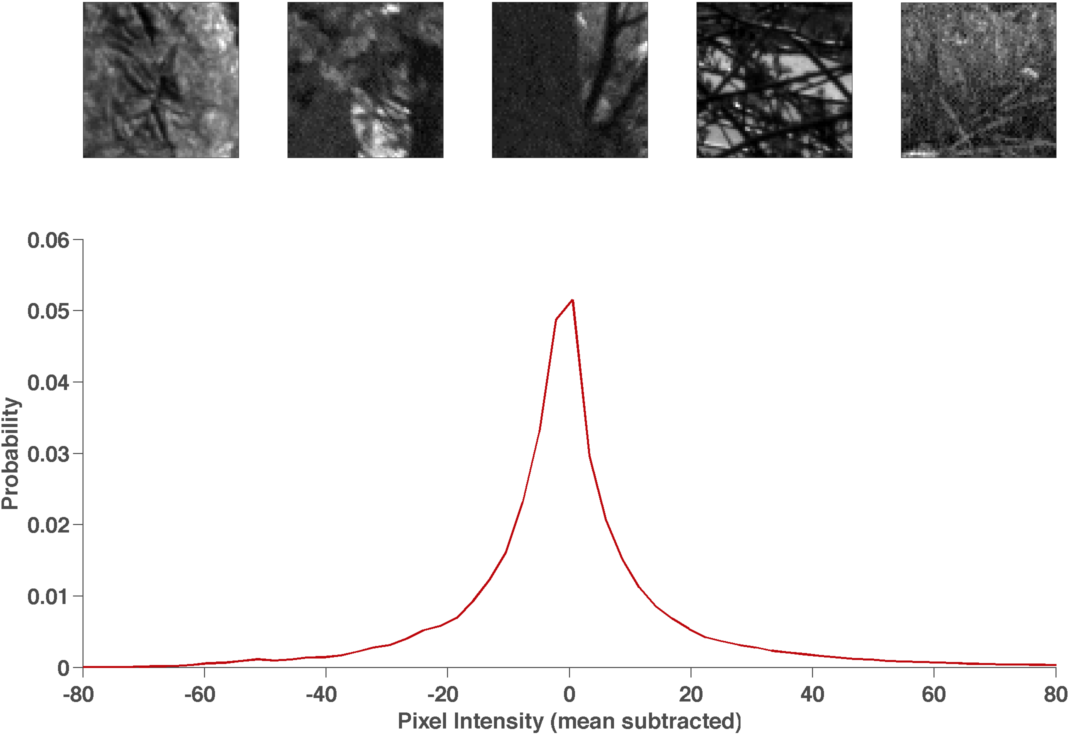
\includegraphics[width=0.7\textwidth]{example_patches.png}
   \caption{Sample natural image patches (top) and probability distribution over single pixel values (bottom)}
\end{center}
\label{fig:ex}
\end{figure*}

\begin{enumerate}
    \item I have generated samples of image patches from a multivariate gaussian distribution with fixed covariance structure, as well as from the van Hateren database. The entropy of a multivariate gaussian is given as $H = \frac{1}{2}\log\left((2\pi e)^k|\Sigma|\right)$, where $k$ is the dimension and $|\Sigma|$ is the determinant of the covariance matrix.
    \item The simplest method of estimating entropy is via kernel density estimation (KDE), where the underlying probability distribution $p(x)$ is approximated given $n$ samples from the distribution. This works well for one-dimensional distributions, and I use KDE as a baseline for comparison with the nearest-neighbor method for 1D distributions.
    \item I implemented the nearest-neighbor algorithm to estimate the entropy from a sampled distribution, as described in Chandler and Field. First, I tested the algorithm on estimating the entropy of a 1D gaussian, which can be confirmed analytically. I also ran the algorithm to estimate the entropy of the distribution of single pixel values.
    \item I am currently working on expanding the nearest-neighbor algorithm to estimate the entropy of high-dimensional distributions. There are some challenges with working in high-dimensions, which I outline in section 5.
    \item I also hope to estimate the entropy of low-dimensional projections of natural images. For example, in class, we have discussed using PCA as a method to reduce the dimensionality of face images. Using this and other algorithms, such as ICA, I plan on generating low-dimensional representations of natural images and then computing entropy in the low-D space (computationally more feasable). This may also yield a method for comparing different reduced descriptions of natural images.
\end{enumerate}

%\section{Evaluation}
%The ultimate goal of this project is to obtain plots of the entropy (in bits per pixel) of image patches for different patch sizes.

%To validate the methods, a comparison of how the various metrics perform when estimating image patches drawn from known distribuitons with fixed statistical structure (white/colored noise) will be used as a baseline for comparison, since the entropy of these distributions is known analytically.

%Once the methods have been validated, entropy estimates of the different measures on natural image patches will be compared. Different curves will be shown for measures of the entropy made using different methods. Another criterion for evaluation is comparing the consistency of different entropy estimates for increasing sample sizes.

%Finally, these results will be compared with recent entropy estimates from the literature [refs].

\section{Preliminary Results}
As described above, I have used a one-dimensional distributions as a baseline for comparing entropy estimation methods. Figure 2 shows the two methods' (kernel density and nearest-neighbor) estimates of the entropy of samples from a univariate normal distribution, along with the (analytically known) true entropy. We see that the estimates converge at similar rates and yield accurate estimates with roughly $10^3$ samples. Estimating with $10^4$ samples already takes a few seconds on my laptop, as computing the nearest-neighbors takes $N^2$ operations.

We can also estimate the entropy on the distribution of pixel intensities drawn from natural images, shown in Figure 3. Here, there is no analytical estimate, but we see that both the kernel density estimate and the nearest-neighbor estimate converge to around 6.5 bits per pixel.

%I have implemented the nearest neighbor algorithm to estimate the entropy of a sampled distribution. In Section (???), I compare this method to a simple kernel density estimate of the entropy of a 1D Gaussian and show how they converge for increasing sample sizes. In Section (???), I apply the same methods to estimate the entropy of samples of single pixel intensities (another 1D distribution). Finally, I have also run the algorithm on N-dimensional distributions, image patches sampled from both whiten oise and natural images. These are discussed in Section ???

%\subsection{1D Distributions}
%To test the implementation of the algorithm, I first tested it on one-dimensional distributions, where the estimate could be compared to estimates via other techniques. Specifically, I tested

%Algorithms for entropy estimation (KDE and NN)

%Estimation of a 1D gaussian (compare to theoretical result)

%Estimation of other 1D distributions with known entropy

%Estimation of distribution of pixel intensities

%Estimation of N-dim gaussian

\section{Current Challenges and Future Work}
The biggest challenge I am currently facing involve computational complexity. The previous work needed to go out to $10^8$ or so samples to get accurate estimates of the entropy for large (8x8) pixel patches. To do this, I think I would have to offload the computation to corn or another cluster. There is also a trade-off between CPU and memory resources, as the distance computation can be done faster in parallel in matlab although it requires a lot of memory for large sample sizes.

While estimating the entropy of the raw distribution of images is a nice first step, I am also very interested in comparing estimates of the reduced descriptions of natural images. By reduced descriptions, I mean doing dimensionality reduction by projecting onto features learned from principal or independent components analysis, for example. I have implemented PCA and ICA on the natural image patches, and a future goal is to estimate the redundancy in these reduced descriptions of natural images.

%\section{Future Work}
%Low-D projections, compute entropy


%\section{Criteria}
%• What is the computer vision problem that you will be investigating? Why is it interesting?

%• What image or video data will you use? If you are collecting new datasets, how do you plan to collect them?

%• What method or algorithm are you proposing? If there are existing implementations, will you use them and how? How do you plan to improve or modify such implementations?

%• Which reading will you examine to provide context and background?

%• How will you evaluate your results? Qualitatively, what kind of results do you expect (e.g. plots or figures)? Quantitatively, what kind of analysis will you use to evaluate and/or compare your results (e.g. what performance metrics or statistical tests)?

%\section{Introduction}

%Please follow the steps outlined below.
%\vspace{3cm}

%-------------------------------------------------------------------------
%\subsection{Language}

%All manuscripts must be in English.

%%-------------------------------------------------------------------------
%\subsection{The ruler}
%The \LaTeX\ style defines a printed ruler which should be present in the
%version submitted for review.  The ruler is provided in order that
%reviewers may comment on particular lines in the paper without
%circumlocution.  If you are preparing a document using a non-\LaTeX\
%document preparation system, please arrange for an equivalent ruler to
%appear on the final output pages.  The presence or absence of the ruler
%should not change the appearance of any other content on the page.  The
%camera ready copy should not contain a ruler.

%\subsection{Mathematics}

%Please number all of your sections and displayed equations.  It is
%important for readers to be able to refer to any particular equation.  Just
%because you didn't refer to it in the text doesn't mean some future reader
%might not need to refer to it.  It is cumbersome to have to use
%circumlocutions like ``the equation second from the top of page 3 column
%1''.  (Note that the ruler will not be present in the final copy, so is not
%an alternative to equation numbers).  All authors will benefit from reading
%Mermin's description of how to write mathematics.%: \url{http://www.cvpr.org/doc/mermin.pdf}.

%\subsection{Miscellaneous}

%\noindent
%Compare the following:\\
%\begin{tabular}{ll}
 %\verb'$conf_a$' &  $conf_a$ \\
 %\verb'$\mathit{conf}_a$' & $\mathit{conf}_a$
%\end{tabular}\\
%See The \TeX book, p165.

%The space after \eg, meaning ``for example'', should not be a
%sentence-ending space. So \eg is correct, {\em e.g.} is not.  The provided
%\verb'\eg' macro takes care of this.

%When citing a multi-author paper, you may save space by using ``et alia'',
%shortened to ``\etal'' (not ``{\em et.\ al.}'' as ``{\em et}'' is a complete word.)
%However, use it only when there are three or more authors.  Thus, the
%following is correct: ``
   %Frobnication has been trendy lately.
   %It was introduced by Alpher~\cite{Alpher02}, and subsequently developed by
   %Alpher and Fotheringham-Smythe~\cite{Alpher03}, and Alpher \etal~\cite{Alpher04}.''

%This is incorrect: ``... subsequently developed by Alpher \etal~\cite{Alpher03} ...''
%because reference~\cite{Alpher03} has just two authors.  If you use the
%\verb'\etal' macro provided, then you need not worry about double periods
%when used at the end of a sentence as in Alpher \etal.

%For this citation style, keep multiple citations in numerical (not
%chronological) order, so prefer \cite{Alpher03,Alpher02,Authors06} to
%\cite{Alpher02,Alpher03,Authors06}.

\begin{figure*}
\begin{center}
%\fbox{\rule{0pt}{2in} \rule{.9\linewidth}{0pt}}
   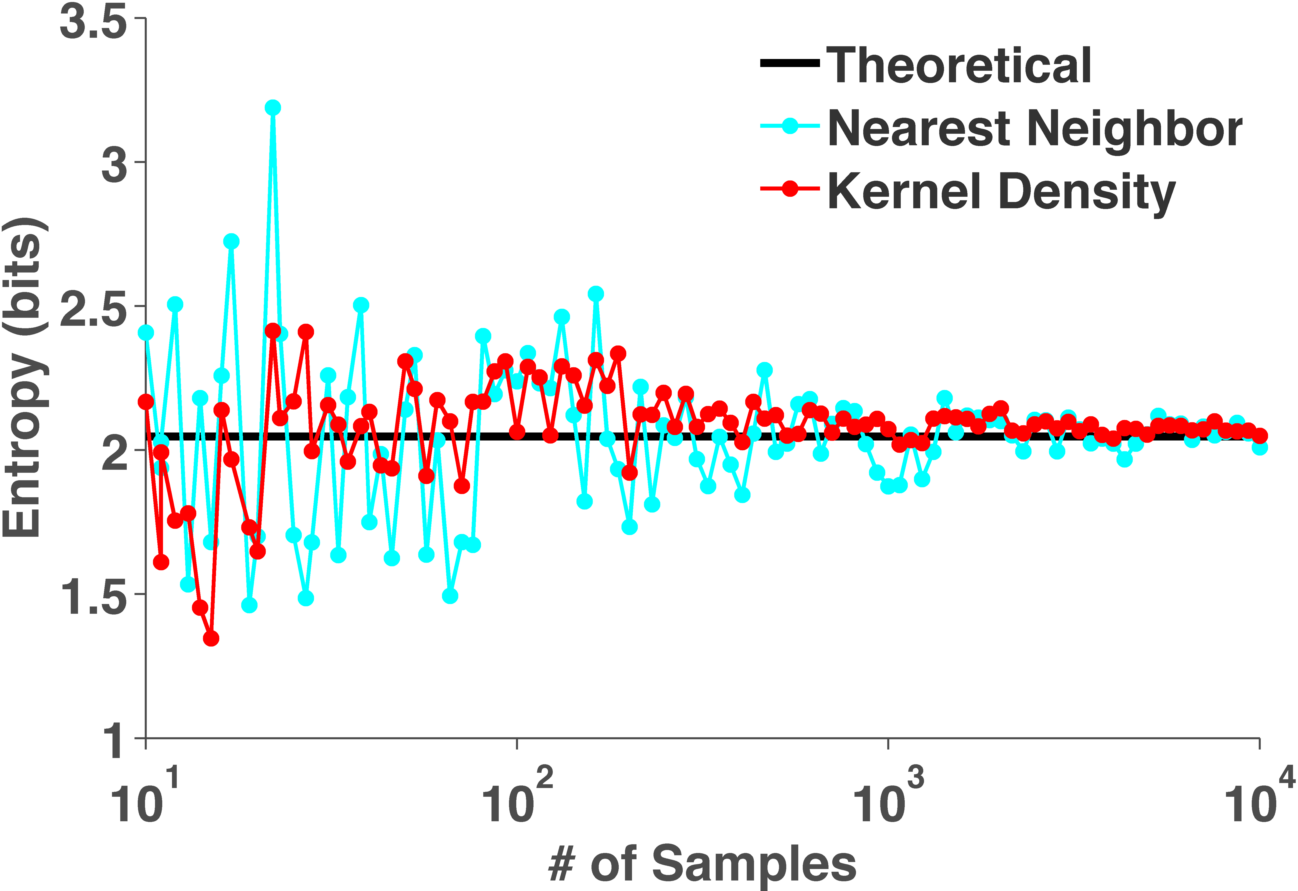
\includegraphics[width=0.8\textwidth]{gaussian_1D.png}
   \caption{Entropy estimation of a normal distribution.}
\end{center}
\label{fig:g1d}
\end{figure*}

\begin{figure*}
\begin{center}
%\fbox{\rule{0pt}{2in} \rule{.9\linewidth}{0pt}}
   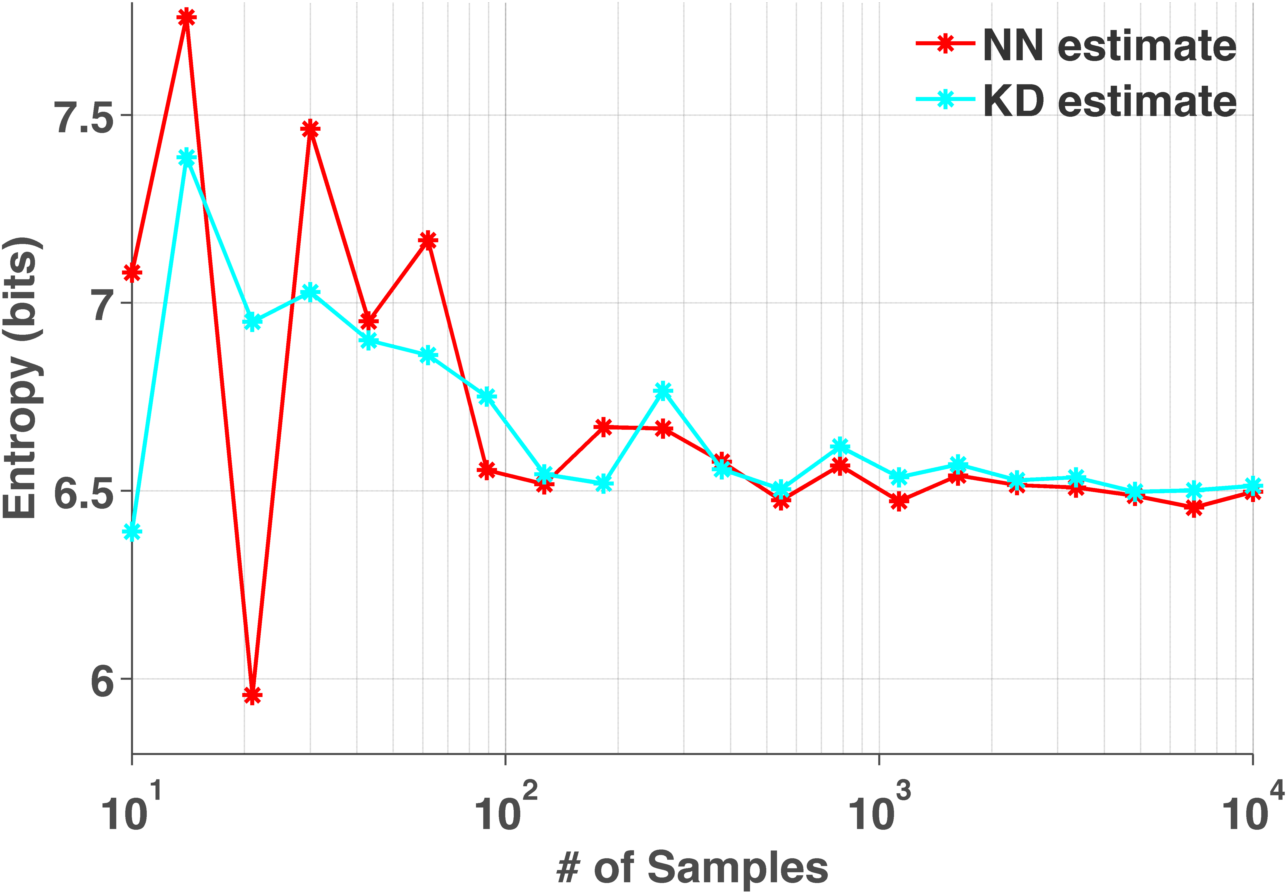
\includegraphics[width=0.8\textwidth]{nongaussian_1D.png}
   \caption{Entropy estimation of the distribution of pixel intensities in natural images.}
\end{center}
\label{fig:ng1d}
\end{figure*}
%------------------------------------------------------------------------
%\begin{table}
%\begin{center}
%\begin{tabular}{|l|c|}
%\hline
%Method & Frobnability \\
%\hline\hline
%Theirs & Frumpy \\
%Yours & Frobbly \\
%Ours & Makes one's heart Frob\\
%\hline
%\end{tabular}
%\end{center}
%\caption{Results.   Ours is better.}
%\end{table}

%-------------------------------------------------------------------------
%\subsection{Illustrations, graphs, and photographs}

%All graphics should be centered.  Please ensure that any point you wish to
%make is resolvable in a printed copy of the paper.  Resize fonts in figures
%to match the font in the body text, and choose line widths which render
%effectively in print.  Many readers (and reviewers), even of an electronic
%copy, will choose to print your paper in order to read it.  You cannot
%insist that they do otherwise, and therefore must not assume that they can
%zoom in to see tiny details on a graphic.

%When placing figures in \LaTeX, it's almost always best to use
%\verb+\includegraphics+, and to specify the  figure width as a multiple of
%the line width as in the example below
%{\small
   %\usepackage[dvips]{graphicx}
   %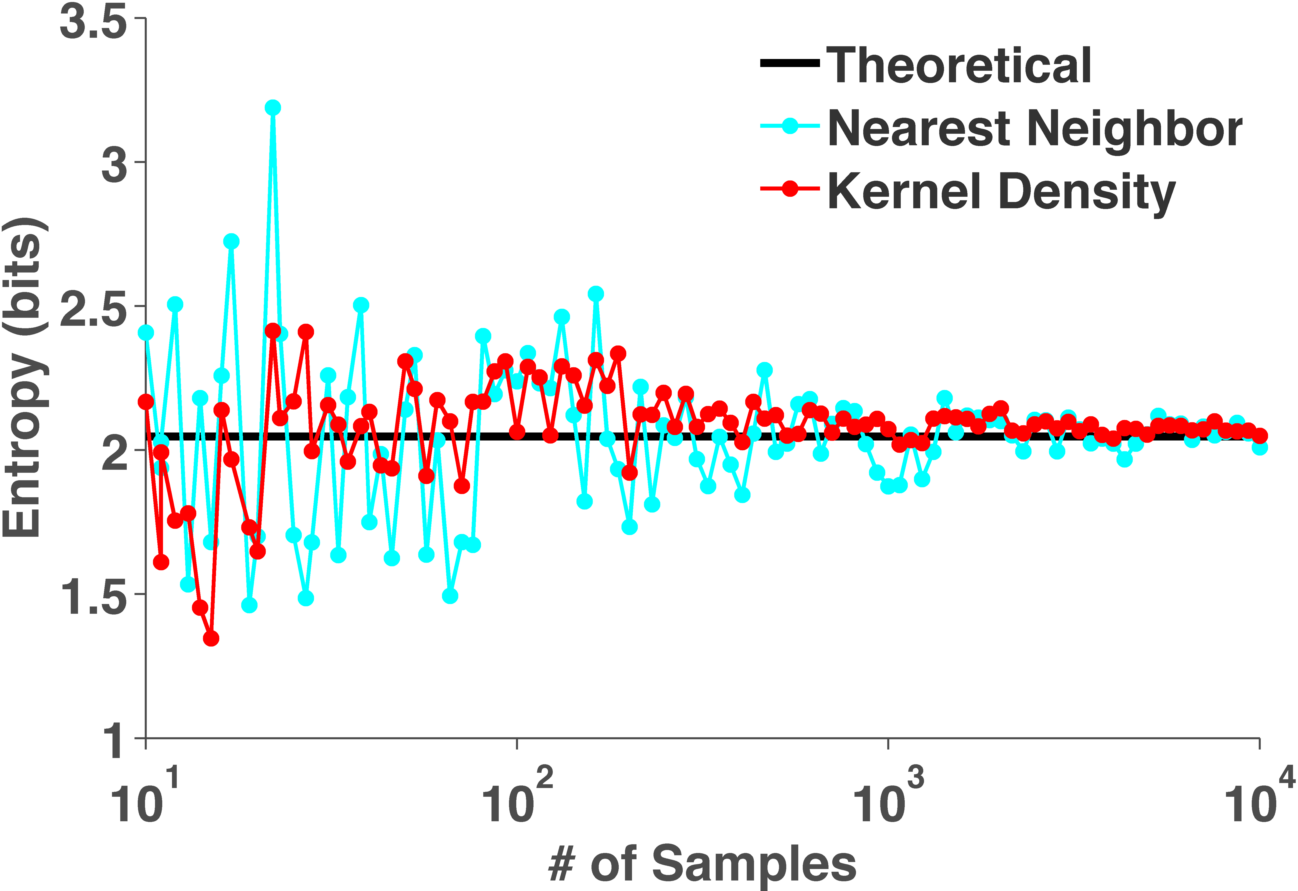
\includegraphics[width=0.99\linewidth]{gaussian_1D.png}
%}


%-------------------------------------------------------------------------
%\subsection{Color}

%Color is valuable, and will be visible to readers of the electronic copy.
%However ensure that, when printed on a monochrome printer, no important
%information is lost by the conversion to grayscale.

{\small
\bibliographystyle{ieee}
\bibliography{egbib}
}

\section{Appendix}
I certify that this project is my own original work. This project is not part of larger work from another class or lab.
%If your course project is part of a larger project from another class or research lab, please fill in this section and clearly spell out the following items:

%\begin{enumerate}
%\item  Explicitly explain what the computer vision components are in this course project;
%\item  Explicitly list out all of your own contributions in this project in terms of:
	%\begin{enumerate}
	%\item ideas
	%\item formulations of algorithms
     %\item software and coding
	%\item designs of experiments
	%\item analysis of experiments
	%\end{enumerate}
%\item Verify and confirm that you (and your partner currently taking CS231A) are the sole author(s) of the writeup.
%Please provide papers, theses, or other documents related to this project so that we can compare with your own writeup.
%\item Please explicitly list out:
	%\begin{enumerate}
	%\item Is this project shared with some other course? If so, what class the project is being shared with (for all members of the team)
	%\item The exact contribution of each person
	%\item The exact portion of the project that is being counted for CS231A
	%\end{enumerate}
	%Failure to do the above is an honor code violation.
%\end{enumerate}
\end{document}
